\documentclass{article}[12pt]

%---------Packages----------
\usepackage{amsmath}
\usepackage{amsfonts}
\usepackage{amssymb}
\usepackage{amsthm}
\usepackage{algorithm,algpseudocode}
\usepackage{enumerate}
\usepackage{graphicx}
\usepackage{fancyhdr}
\usepackage{tikz}
\usepackage{pgfplots}

\usetikzlibrary{decorations.pathreplacing}

% for drawing pretty pictures
\pgfplotsset{compat=1.10}
\usepgfplotslibrary{fillbetween}
\usetikzlibrary{patterns}

\usepackage{tikz}
\usetikzlibrary{3d}
\usetikzlibrary{calc}

%% ------------------------------------------------------------
%% PACKAGES
%% ------------------------------------------------------------

%% For \circledast
\usepackage{amssymb,amsfonts}

%% For \mathscr
\usepackage[mathscr]{eucal}

%% For \llbracket and \rrbracket, \varoast, \varoslash
\usepackage{stmaryrd}

%% For \boldsymbol
\usepackage{amsbsy}

%% For \bm (bold math)
\usepackage{bm}

%% For \set, \Set
\usepackage{braket}

%% ------------------------------------------------------------
%% TENSOR NOTATION MACROS
%% ------------------------------------------------------------

%% --- Extras ---
% Transpose
\newcommand{\Tra}{{\sf T}} 
\newcommand{\parens}[1]{(#1)}
\newcommand{\Parens}[1]{\left(#1\right)}
\newcommand{\dsquare}[1]{\llbracket #1 \rrbracket}
\newcommand{\Dsquare}[1]{\left\llbracket #1 \right\rrbracket}
\newcommand{\curly}[1]{\{ #1 \}}
\newcommand{\Curly}[1]{\left\{ #1 \right\}}
\newcommand{\Real}{\mathbb{R}}
\newcommand{\qtext}[1]{\quad\text{#1}\quad}

%% --- Vectors ---
% vector
\newcommand{\V}[2][]{{\bm{#1\mathbf{\MakeLowercase{#2}}}}} 
% element of vector
\newcommand{\VE}[3][]{#1{\MakeLowercase{#2}}_{#3}} 
% vector in series
\newcommand{\Vn}[3][]{{\bm{#1\mathbf{\MakeLowercase{#2}}}}^{(#3)}} 
% transposed vector in series
\newcommand{\VnTra}[3][]{{\bm{#1\mathbf{\MakeLowercase{#2}}}}^{(#3)\Tra}} 
% element of vector in series
\newcommand{\VnE}[4][]{#1{\MakeLowercase{#2}}^{(#3)}_{#4}} 

%% --- Matrices ---
% matrix
\newcommand{\M}[2][]{{\boldsymbol{#1\mathbf{\MakeUppercase{#2}}}}} 
% matrix in series
\newcommand{\Mn}[3][]{{\boldsymbol{#1\mathbf{\MakeUppercase{#2}}}}^{(#3)}} 
% transposed matrix in series 
\newcommand{\MnTra}[4][]{{\bm{#1\mathbf{\MakeUppercase{#2}}}}^{(#3)\Tra}} 
% matrix column
\newcommand{\MC}[3][]{\V[#1]{#2}_{#3}} 
% column of matrix in series
\newcommand{\MnC}[4][]{\Vn[#1]{#2}{#3}_{#4}} 
% transposed column of matrix in series
\newcommand{\MnCTra}[4][]{\VnTra[#1]{#2}{#3}_{#4}} 
% matrix element
\newcommand{\ME}[3][]{#1{\MakeLowercase{#2}}_{#3}} 
% element of matrix in series
\newcommand{\MnE}[4][]{#1{\MakeLowercase{#2}}^{(#3)}_{#4}} 

%% --- Tensors ---
% tensor
\newcommand{\T}[2][]{\boldsymbol{#1\mathscr{\MakeUppercase{#2}}}} 
% tensor slide
\newcommand{\TS}[3][]{\M[#1]{#2}_{#3}}
% tensor element
\newcommand{\TE}[3][]{#1{\MakeLowercase{#2}}_{#3}}
% matricized tensor
\newcommand{\Mz}[3][]{\M[#1]{#2}_{(#3)}}
% tensor in series
\newcommand{\Tn}[3][]{\boldsymbol{#1\mathscr{\MakeUppercase{#2}}}^{(#3)}} 


%% --- Operators ---
% outer product
\newcommand{\Oprod}{\circ} 
% Kronecker product
\newcommand{\Kron}{\otimes} 
% Khatri-Rao product
\newcommand{\Khat}{\odot} 
% Hadamard (elementwise multiply)
\newcommand{\Hada}{\ast} 
\newcommand{\BigHada}{\mathop{\mbox{\fontsize{18}{19}\selectfont $\circledast$}}} 
% Elementwise divide
\newcommand{\Divi}{\varoslash}
%% ------------------------------------------------------------

%----------PageStyleStuff----------
\textwidth=6.5in
\textheight=8.0in
\topmargin=0in
\oddsidemargin=0in
\evensidemargin=0in

\title{Efficient Computation of Tucker Decomposition of Correlation-Based Tensors}
\author{Bill Xu \medskip \\ Advisor: Grey Ballard \\ in collaboration with Robert Lyday, and Paul Laurienti}
\begin{document}

\maketitle

%\section{Tucker Decomposition}

%\begin{figure}
%\centering
%%!TEX root = ../paper.tex

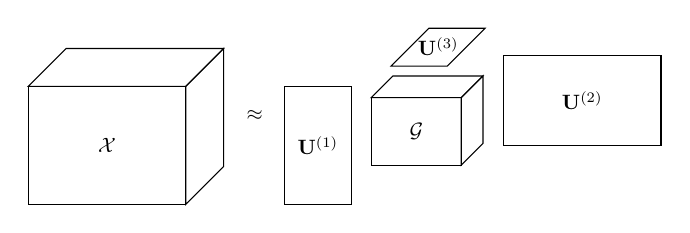
\begin{tikzpicture}[scale=0.5,namenode/.style={scale=.75}]

%\draw[help lines] (0,0) grid (20,6);

% Set relative dimensions of X
\def\ix{4} %<- Second dimension of tensor
\def\iy{3} %<- First dimension of tensor
\def\iz{2.5} %<- Third dimension of tensor

% Set relative dimensions of G
\def\corescale{1.75}
\def\rx{\ix/\corescale}
\def\ry{\iy/\corescale}
\def\rz{\iz/\corescale}

%\draw[help lines,step=.2] (0,0) grid (17,5);

% X Tensor
\coordinate (XFrontLowerLeft) at (0,0);
\draw (XFrontLowerLeft) rectangle ++ (\ix,\iy); % Front
\begin{scope}[shift={(XFrontLowerLeft)},canvas is zx plane at y=\iy,rotate=90]
  \draw (0,0) rectangle ++ (\ix,\iz); % Top
\end{scope}
\begin{scope}[shift={(XFrontLowerLeft)},canvas is zy plane at x=\ix,rotate=90]
  \draw (0,0) rectangle ++ (\iy,\iz); % Right
\end{scope}
\node[namenode] at ($(XFrontLowerLeft) + (0.5*\ix, 0.5*\iy)$)  {${\cal X}$};

% \approx
\coordinate (ApproxCtr) at ($(XFrontLowerLeft) + (\ix+0.4*\iz,0.75*\iy) + (0.75,0)$);
\node[namenode] at (ApproxCtr) {$\approx$};

% U1
\coordinate (U1LowerLeft) at ($(ApproxCtr) - (0,0.75*\iy) + (0.75,0)$);
\draw (U1LowerLeft) rectangle ++ (\ry,\iy);
\node[namenode] at ($(U1LowerLeft)+(0.5*\ry, 0.5*\iy)$)  {$\mathbf{U}^{(1)}$};

% G
\coordinate (GFrontLowerLeft) at ($(U1LowerLeft) + (\ry+0.5,1)$);
\draw (GFrontLowerLeft) rectangle ++ (\rx,\ry);
\begin{scope}[shift={(GFrontLowerLeft)},canvas is zx plane at y=\ry,rotate=90]
  \draw (0,0) rectangle ++ (\rx,\rz);
\end{scope}
\begin{scope}[shift={(GFrontLowerLeft)},canvas is zy plane at x=\rx,rotate=90]
  \draw (0,0) rectangle ++ (\ry,\rz);
\end{scope}
\node[namenode] at ($(GFrontLowerLeft)+(0.5*\rx,.5*\ry)$)  {${\cal G}$};

%U2
\coordinate (U2LowerLeft) at ($(GFrontLowerLeft) + (\rx+\rz*0.4+0.5,0.5)$);
\draw (U2LowerLeft) rectangle ++ (\ix,\rx); % Right
\node[namenode] at ($(U2LowerLeft)+(0.5*\ix,0.5*\rx)$)  {$\mathbf{U}^{(2)}$};

%U3
\coordinate (U3LowerLeft) at ($(GFrontLowerLeft) + (0.5,\ry+.8)$);
\begin{scope}[shift={(U3LowerLeft)},canvas is zx plane at y=0,rotate=90]
  \draw (0,0) rectangle ++ (\rz,\iz); % Top
\end{scope}
\node[namenode] at ($(U3LowerLeft)+(1.2,0.5)$) {$\mathbf{U}^{(3)}$};

\end{tikzpicture}


%%% Local Variables: 
%%% mode: latex
%%% TeX-master: "../paper"
%%% End: 

%\caption{Tucker Model}
%\end{figure}

%Correlation among different areas in the brain has been an interested topic in neuroscience for long. However some compromise must be made on the granularity of brain activity scan when storing and processing data. As the computation and storage power evolve, we are increasingly interested in discovering brain data in higher accuracy and larger scale. In this research we aim to (1) Find an efficient algorithm to reduce dimension of correlation activity tensor. (2) Find possible scientific questions that demonstrate advantage of using finer granularity of data. 

\begin{abstract}
The Tucker decomposition is a generalization of the matrix singular value decomposition to tensors, which are multidimensional arrays.
We seek to apply the decomposition as a dimension reduction technique in order to analyze large functional magnetic resonance imaging (f-MRI) datasets of human brains.
Neuroscientists are particularly interested in correlation among different areas in the brain, but computing and storing pairwise correlations between all pairs of brain areas can be infeasible, especially when the data set includes multiple participants and multiple trials.
The current practice is to downsample the data in order to reduce the number of brain areas in the data, but this process loses information.
We show that the dimension reduction via Tucker decomposition can be computed without explicitly computing and storing all correlations, making data analysis with the original granularity feasible and efficient.
We demonstrate the advantage of using the full granularity to answer scientific questions about the data, including classifying participants across multiple trials.
\end{abstract}


\section{Introduction}
\subsection{Background}
Correlation between different areas of brains has been topic of interest in neuroscience for a long time. One of the methods in brain imaging is Functional Magnetic Resonance Imaging (f-MRI), which measures brain activity by detecting changes of blood flow. While scanning brains using f-MRI, the unit of measurement for voxels is on the scale of cubic nanometers. For example, a typical available granularity is $4\text{nm} \times 4\text{nm} \times 4\text{nm} $, which we will refer to as Voxel-based data.  Because of the fine granularity, the data requires huge space of memory to store and time to process. Alternatively, neuroscientists have manually defined 268 anatomically specific regions, each of which combines different sets of voxels to save memory at a cost of reducing granularity. We call this coarser-grained representation Region-based data. Our research addresses two related problems: (1) Can we improve efficiency and reduce memory usage when processing f-MRI data? (2) What are the advantages of using Voxel-based over Region-based data in answering neuroscience questions?

\subsection{Preliminaries}

\subsubsection{Singular Vector Decomposition}
The Singular Value Decomposition (SVD) is a technique for linear dimensionality reduction to project high dimensional data to a lower dimensional space.  In our research, SVD decomposes a flattened Neural Activity Tensor into matrix multiplication of left singular vectors, singular values, and right singular vectors. In this way we can map high dimensional f-MRI data into a low dimensional matrix of left singular vectors.

\subsubsection{Machine Learning Models}

We have implemented multiple machine learning models to experiment on scientific questions, including Random Forest, Gradient Boosting Decision Trees and K-Nearest Neighbors and Generalized Linear Regression. A random forest \cite{RF} is a meta estimator that fits a number of decision tree classifiers on various sub-samples of the dataset and uses averaging to improve the predictive accuracy and control over-fitting. Gradient Boosting \cite{GBDT} builds an additive model in a forward stage-wise fashion; it allows for the optimization of arbitrary differentiable loss functions. Both of them exploit ensemble to improve predictive accuracy and generalizability. Gradient Boosting Decision Trees builds on weak learners (shallow trees) while Random Forest aims at fully growing decision trees. Therefore GBDT tends to reduce bias while Random Forest reduces variance. 




\section{Data}
The data we use comes from f-MRI (Functional Magnetic Resonance Imaging) brain image scans. Such scans of brain take places at certain intervals (or timesteps) for each participant. Therefore we can store the data in a 3 dimensional tensor called Activity Tensor $\T{A}$.  Beyond that, we need several transformation based on $\T{A}$. We define a Static Correlation Tensor as $\T{S}$, Window Activity Tensor $\cal W$, Dynamic Correlation Tensor $\cal C$. Besides $P$ is number of participants, $A$ is number of brain regions (areas), $T$ is number of time points, $W$ is width of window, $N=T-W+1$ is number of windows

	
\subsection{Activity Tensor}
In either region based or voxel based methods, the activity tensor, ${\T A}$ of the brain data is a three way tensor of Area ($A$), Time($T$) and Participant($P$). The entry $\TE{A}{ijk}$  is a record of either regional or voxel brain data of area $i$,  at time $j$ for participant $j$.


\begin{center}
	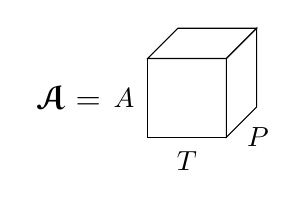
\begin{tikzpicture}
	\pgfmathsetmacro{\cubex}{1}
	\pgfmathsetmacro{\cubey}{1}
	\pgfmathsetmacro{\cubez}{1}
	\draw[black] (0,0,0) -- ++(-\cubex,0,0) -- ++(0,-\cubey,0) -- ++(\cubex,0,0) -- cycle;
	\draw[black] (0,0,0) -- ++(0,0,-\cubez) -- ++(0,-\cubey,0) -- ++(0,0,\cubez) -- cycle;
	\draw[black] (0,0,0) -- ++(-\cubex,0,0) -- ++(0,0,-\cubez) -- ++(\cubex,0,0) -- cycle;
	\node at (-1.3,-0.5) {$A$};
	\node at (-0.5,-1.3) {$T$};
	\node at (0.4, -1.0) {$P$};
	\node at (-2,-0.5) {\large ${\T A} = $};
	\end{tikzpicture}
\end{center}
For the purpose of computing correlation, we define ${\T[\hat]{A}}$ from $\T{A}$ by shifting each time series towards center and normalizing.

\begin{equation*}
{\T[\hat]{A}}(a,:,p) = \frac{{\T A}(a,:,p) - \overline{{\T A}(a,:,p)}}{\|{\T A}(a,:,p) - \overline{{\T A}(a,:,p)}\|_2}
\end{equation*}


\subsection{Static Analysis Correlation Tensor}
The static analysis correlation tensor ${\cal S}$ is a three way tensor ($A$ by $A$ by $P$).  ${\cal S}_{ijk}$ is the statistical correlation between two areas fibers $A_{ik}$ and $A_{jk}$ over $T$ for participant $k$.  The statistical correlation of two vectors $x$ and $y$ is defined by 

\begin{equation*}
\text{corr}(\V{x},\V{y}) = \frac{\sum_{i=1}^{n} (\VE{x}{i} - \overline{x})(\VE{y}{i} - \overline{y})}
{\sqrt{\sum_{i=1}^{n} (\VE{x}{i} - \overline{x})^2} \sqrt{\sum_{i=1}^n (\VE{y}{i} - \overline{y})^2}} 
= \mathbf{\hat{\V x}}^T\mathbf{\hat{\V y}}
\end{equation*}
where $\mathbf{\hat{\V x}} = \frac{\mathbf{\V x} - \overline{x} \mathbf{1}}{\|\mathbf{\V x} - \overline{x} \mathbf{1}\|_2}$. Thus, 

\begin{center}
	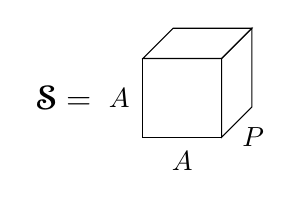
\begin{tikzpicture}
	\pgfmathsetmacro{\cubex}{1}
	\pgfmathsetmacro{\cubey}{1}
	\pgfmathsetmacro{\cubez}{1}
	\draw[black] (0,0,0) -- ++(-\cubex,0,0) -- ++(0,-\cubey,0) -- ++(\cubex,0,0) -- cycle;
	\draw[black] (0,0,0) -- ++(0,0,-\cubez) -- ++(0,-\cubey,0) -- ++(0,0,\cubez) -- cycle;
	\draw[black] (0,0,0) -- ++(-\cubex,0,0) -- ++(0,0,-\cubez) -- ++(\cubex,0,0) -- cycle;
	\node at (-1.3,-0.5) {$A$};
	\node at (-0.5,-1.3) {$A$};
	\node at (0.4, -1.0) {$P$};
	\node at (-2,-0.5) {\large ${\T S} = $};
	\end{tikzpicture}
\end{center}
where ${\T S}(:,:,p) = \hat{\T A}(:,:,p) \hat{\T A}(:,:,p)^T$.



\subsection{Dynamic Analysis Correlation Tensor}
To calculate correlation between areas of a given participant at a specific time $n$, one should not use area fibers over full time, ${\T A}(a,:,p)$, to compute correlation. Instead, we propose sliding windows at time $n$ with size $W$ to compute correlation.


\subsubsection{Windowed Activity Tensor}
The windowed activity tensor ${\T W}$  is a four way tensor of Area ($A$), Time ($W$), Participant ($P$), and Window ($N$) .  Entry ${\T W}_{ijkn}$ is a record of either regional or voxel brain data of area $i$,  at window time $j$ for participant $j$ and window index $n$.

\begin{center}
	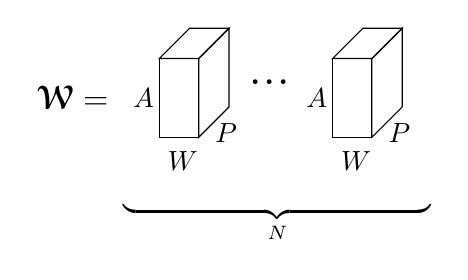
\begin{tikzpicture}[level/.style={},decoration={brace,mirror,amplitude=7}]
	\pgfmathsetmacro{\cubex}{0.5}
	\pgfmathsetmacro{\cubey}{1}
	\pgfmathsetmacro{\cubez}{1}
	\draw[black] (0,0,0) -- ++(-\cubex,0,0) -- ++(0,-\cubey,0) -- ++(\cubex,0,0) -- cycle;
	\draw[black] (0,0,0) -- ++(0,0,-\cubez) -- ++(0,-\cubey,0) -- ++(0,0,\cubez) -- cycle;
	\draw[black] (0,0,0) -- ++(-\cubex,0,0) -- ++(0,0,-\cubez) -- ++(\cubex,0,0) -- cycle;
	\node at (0.9,-0.3) {\huge ...};
	\draw[black] (2.2,0,0) -- ++(-\cubex,0,0) -- ++(0,-\cubey,0) -- ++(\cubex,0,0) -- cycle;
	\draw[black] (2.2,0,0) -- ++(0,0,-\cubez) -- ++(0,-\cubey,0) -- ++(0,0,\cubez) -- cycle;
	\draw[black] (2.2,0,0) -- ++(-\cubex,0,0) -- ++(0,0,-\cubez) -- ++(\cubex,0,0) -- cycle;
	\node at (-0.7,-0.5) {$A$};
	\node at (-0.2,-1.3) {$W$};
	\node at (0.35, -0.95) {$P$};
	\node at (1.5,-0.5) {$A$};
	\node at (2,-1.3) {$W$};
	\node at (1,-2) {$\underbrace{\phantom{aaaaaaaaaaaaaaaaaaaaa}}_{N}$}; % edit this to stretch across
	%\draw [decorate] ([yshift=-5mm]1.0) --1.2[below=3mm]{$n_1$} ([yshift=-5mm]1.3);
	\node at (2.55, -0.95) {$P$};
	\node at (-1.6,-0.5) {\large ${\T W} = $};
	\end{tikzpicture}
\end{center}
Similar to its static counterpart, we define $\T [\hat]{X}$ $\hat{\T{W}}$ from $\T{W}$ by shifting and normalizing towards center.

\begin{equation*}
{\T [\hat]{W}}(a,:,p,n) = \frac{{\T W}(a,:,p,n) - \overline{{\T W}(a,:,p,n)}}{\|{\T W}(a,:,p,n) - \overline{{\T W}(a,:,p,n)}\|_2}
\end{equation*}





\subsubsection{Correlation Tensor}
The dynamic correlation tensor ${\T C}$ is a four way tensor ($A$ by $A$ by $P$ by $N$). The entry ${\T C}_{ijpn}$ is the statistical correlation between two areas $i$ and $j$ for participant $k$ at time $n$.

\begin{center}
	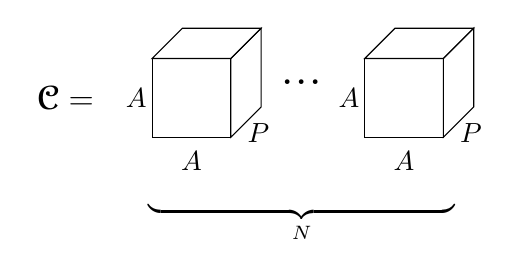
\begin{tikzpicture}
	\pgfmathsetmacro{\cubex}{1}
	\pgfmathsetmacro{\cubey}{1}
	\pgfmathsetmacro{\cubez}{1}
	\draw[black] (0.1,0,0) -- ++(-\cubex,0,0) -- ++(0,-\cubey,0) -- ++(\cubex,0,0) -- cycle;
	\draw[black] (0.1,0,0) -- ++(0,0,-\cubez) -- ++(0,-\cubey,0) -- ++(0,0,\cubez) -- cycle;
	\draw[black] (0.1,0,0) -- ++(-\cubex,0,0) -- ++(0,0,-\cubez) -- ++(\cubex,0,0) -- cycle;
	\node at (1,-0.3) {\huge ...};
	\draw[black] (2.8,0,0) -- ++(-\cubex,0,0) -- ++(0,-\cubey,0) -- ++(\cubex,0,0) -- cycle;
	\draw[black] (2.8,0,0) -- ++(0,0,-\cubez) -- ++(0,-\cubey,0) -- ++(0,0,\cubez) -- cycle;
	\draw[black] (2.8,0,0) -- ++(-\cubex,0,0) -- ++(0,0,-\cubez) -- ++(\cubex,0,0) -- cycle;
	\node at (-1.1,-0.5) {$A$};
	\node at (-0.4,-1.3) {$A$};
	\node at (0.45, -0.95) {$P$};
	\node at (1.6,-0.5) {$A$};
	\node at (2.3,-1.3) {$A$};
	\node at (3.15, -0.95) {$P$};
	\node at (-2,-0.5) {\large ${\T C} = $};
	\node at (1,-2) {$\underbrace{\phantom{aaaaaaaaaaaaaaaaaaaaa}}_{N}$}; % edit this to stretch across
	\end{tikzpicture}
	
\end{center}
where ${\T C}(:,:,p,n) = \hat{\T W}(:,:,p,n) \hat{\T W}(:,:,p,n)^T$, and ${\T C}(i,j,p,n)$ is the inner product of two vectors $\hat{\T W}(i,:,p,n)$ and $\hat{\T W}(j,:,p,n)$

\section{Algorithms}

\subsection{Static Analysis Correlation Tensor}
In case where we view tensor $\T {S}$ as correlation of areas for participants over \textbf{all} time points of $\T {A}$, the algorithm is presented as Algorithm \ref{alg:static}. Notice that certain time series vectors must be centered and normalized before used to calculate correlation matrix.


%\begin{center}
%	\begin{tikzpicture}[level/.style={},decoration={brace,mirror,amplitude=7}]
%	\pgfmathsetmacro{\cubex}{0.5}
%	\pgfmathsetmacro{\cubey}{1}
%	\pgfmathsetmacro{\cubez}{1}
%	\draw[black] (0,0,0) -- ++(-\cubex,0,0) -- ++(0,-\cubey,0) -- ++(\cubex,0,0) -- cycle;
%	\draw[black] (0,0,0) -- ++(0,0,-\cubez) -- ++(0,-\cubey,0) -- ++(0,0,\cubez) -- cycle;
%	\draw[black] (0,0,0) -- ++(-\cubex,0,0) -- ++(0,0,-\cubez) -- ++(\cubex,0,0) -- cycle;
%	\node at (0.9,-0.3) {\huge ...};
%	\draw[black] (2.2,0,0) -- ++(-\cubex,0,0) -- ++(0,-\cubey,0) -- ++(\cubex,0,0) -- cycle;
%	\draw[black] (2.2,0,0) -- ++(0,0,-\cubez) -- ++(0,-\cubey,0) -- ++(0,0,\cubez) -- cycle;
%	\draw[black] (2.2,0,0) -- ++(-\cubex,0,0) -- ++(0,0,-\cubez) -- ++(\cubex,0,0) -- cycle;
%	\node at (-0.7,-0.5) {$A$};
%	\node at (-0.2,-1.3) {$W$};
%	\node at (0.35, -0.95) {$P$};
%	\node at (1.5,-0.5) {$A$};
%	\node at (2,-1.3) {$W$};
%	\node at (1,-2) {$\underbrace{\phantom{aaaaaaaaaaaaaaaaaaaaa}}_{N}$}; % edit this to stretch across
%	%\draw [decorate] ([yshift=-5mm]1.0) --1.2[below=3mm]{$n_1$} ([yshift=-5mm]1.3);
%	\node at (2.55, -0.95) {$P$};
%	\node at (-1.6,-0.5) {\large ${\T W} = $};
%	\end{tikzpicture}
%\end{center}

\begin{algorithm}
\caption{Static Analysis Correlation Tensor}
\label{alg:static}
\begin{algorithmic}[1]
\Require $\T{A}$ is original 3-way data tensor with dimension $A \times T \times P$
 \For{\texttt{p = 1:P}}
   \For{\texttt{a = 1:A}}
      \State \texttt{$\T [\hat]{A}(a,:,p) = \T {A}(a,:,p)  - \overline{{\T A}(a,:,p)} $ } \hfill \Comment{center time series vector}
      \State \texttt{$\T [\hat]{A}(a,:,p) = \T [\hat]{A}(a,:,p)/ {\|{\T [\hat]A}(a,:,p)\|_2}$ }   \hfill \Comment{normalize time series vector}
   \EndFor
   \State \texttt{$\T {S}(:,:,p) = {\T [\hat]A}(:,:,p) {\T [\hat]A}(:,:,p)^T$ } \hfill \Comment{calculate correlation matrix}
 \EndFor
\end{algorithmic}
\end{algorithm}




\subsection{Dynamic Analysis Correlation Tensor}
Our primary goal is to compute the left singular vectors of $\Mz{C}{4}$, the participant-mode unfolding of dynamic correlation tensor $\T {C}$. Thus, an intuitive algorithm is based on our experience in the previous section: explicitly compute windowed activity tensor $\T {W}$, then calculate the corresponding correlation tensor $\T {C}$, and finally form the left singular vectors of $\Mz{C}{4}$.
This approach is presented as Algorithm \ref{alg:explicit}.

\begin{figure}  \centering
	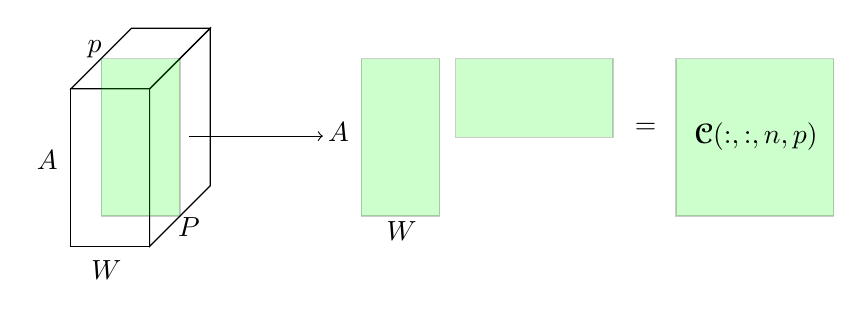
\begin{tikzpicture}[level/.style={},decoration={brace,mirror,amplitude=7}]
	\pgfmathsetmacro{\cubex}{1}
	\pgfmathsetmacro{\cubey}{2}
	\pgfmathsetmacro{\cubez}{2}
	\draw[black] (0,0,0) -- ++(-\cubex,0,0) -- ++(0,-\cubey,0) -- ++(\cubex,0,0) -- cycle;
	\draw[black] (0,0,0) -- ++(0,0,-\cubez) -- ++(0,-\cubey,0) -- ++(0,0,\cubez) -- cycle;
	\draw[black] (0,0,0) -- ++(-\cubex,0,0) -- ++(0,0,-\cubez) -- ++(\cubex,0,0) -- cycle;
         \draw [draw=black, fill=green,  opacity=0.2]
         (0,0,-1) -- ++(-\cubex,0,0) -- ++(0,-\cubey,0) -- ++(\cubex,0,0) -- cycle;
	\node at (-1.3,-0.9) {$A$};
	\node at (-0.55,-2.3) {$W$};
	\node at (0.5, -1.75) {$P$};
	\node at (-0.7,0.5) {$p$};
	\draw[arrows=->](0.5,-0.6)--(2.2, -0.6);
	\draw [draw=black, fill=green,  opacity=0.2]
         (3.3,0,-1) -- ++(-\cubex,0,0) -- ++(0,-\cubey,0) -- ++(\cubex,0,0) -- cycle;
        \draw [draw=black, fill=green,  opacity=0.2]
         (3.5,0,-1) -- ++(0,-\cubex,0) -- ++(\cubey,0,0) -- ++(0,\cubex,0) -- cycle;
         \node at (6.3,-0.5) {$= $};
         \draw [draw=black, fill=green,  opacity=0.2] (8.3,0,-1) -- ++(-\cubey,0,0) -- ++(0,-\cubey,0) -- ++(\cubey,0,0) -- cycle;
         %\node at (7.7, -0.2) {C_{n}^{p}}
         \node at (7.7 ,-0.6) {$\T {C}(:,:,n,p)$};
	\node at (2.4,-0.55) {$A$};
	\node at (3.2,-1.8) {$W$};
	
	\end{tikzpicture}
	\caption{Subtensor corresponding to correlation of participant p and window n}
\end{figure}



\begin{algorithm}
\caption{Left Singular Vector of Dynamic Analysis Correlation Tenso r(explicit)}
\label{alg:explicit}
\begin{algorithmic}[1]
\Require $\T{A}$ is original 3-way data tensor with dimension $A \times T  \times P$
\Require $W$ is the window size in windowed activity tensor
        \State \texttt{N = T - W + 1 } \hfill \Comment{number of windows}
	\For{\texttt{p = 1:P}}
 		\For{\texttt{n = 1:N}}
   			\State $\M{W} = \T{A}(:,n:n+W-1,p)$
			\For{\texttt{a = 1:A}}
				\State \texttt{$\M[\hat]{W}(a,:) = \M{W}(a,:)  - \overline{\M{W}(a,:)} $ } \hfill \Comment{center (windowed) time series vector}
				\State \texttt{$\M[\hat]{W}(a,:) = \M[\hat]{W}(a,:)/ {\|{\M[\hat]W}(a,:)\|_2}$ }   \hfill \Comment{normalize (windowed) time series vector}
			\EndFor
			\State \texttt{$\T {C}(:,:,n,p) = \M[\hat]{W} \M[\hat]{W}^\Tra$ } \hfill \Comment{calculate 2D slice of dynamic correlation tensor}
		\EndFor
	\EndFor
\State $\M{G} = \Mz{C}{4}\Mz{C}{4}^\Tra$ \hfill \Comment{Compute Gram matrix of participant mode unfolding}
\State $[\M{U}, \M{\Lambda}] = \text{EVD}(\M{G})$ \hfill \Comment{$\M U$ := eigenvectors; $\M \Lambda$ := eigenvalues}
\State \texttt{Sort $\M{U},\M{\Lambda}$ by descending order of $\M{\Lambda}$} 
\State $\M{\Sigma} = \sqrt{\M{\Lambda}}$ \hfill \Comment{singular values of $\Mz{C}{4}$, $\M U$ are left singular vectors}
\end{algorithmic}
\end{algorithm}





There are two steps involved in this algorithm: (1) Computing correlation tensor $\T {C}$, which costs $A^2WPN$ flops because for each of N windows, and for each of P participants, there is a need to compute a matrix multiplication of shape $A \times W$ and its transpose, and such multiplication costs $A^2 W$ flops (since the result is symmetric). (2) Computing the SVD via and EVD of the Gram matrix to recover left singular vectors. Since $\Mz{C}{4}$ is a matrix of size $P \times (A \times A \times N)$,  computing the Gram matrix costs $A^2 P^2  N$ flops. 

The space complexity is attributed to (1) Activity tensor $\T A$ which takes $A T P$ unit of space. (2) Correlation tensor $\T C$ which takes $A^2  N P$ unit of space.



\bigbreak

Alternatively, we propose an approach that implicitly calculates the Gram matrix $\M {G}$, resulting in both computational and spatial efficiency particularly when $A$ is large. The implicit algorithm is based on following derivation:
\begin{align*}
 (\Mz{C}{4} \Mz{C}{4}^T)_{ij} &= <\M{M}_i, \M{M}_j> \\ &= \sum_{n}^{N} <C_n^i, C_n^j>
\\ &=  \sum_{n}^{N} <{A_n^i }{A_n^i}^T,{A_n^j}{A_n^j}^T >
\\ &=  \sum_{n}^{N} <{A_n^i }^T{A_n^i},{A_n^j}^T{A_n^j}>
\\ &=  \sum_{n}^{N} \| {A_n^i}^T{A_n^j} \|_F^2
\end{align*}
where $C_n^i = \T {C}(:,:,n,i)$ and $A_n^i = \T {A}(:,n:n+W-1,i)$. 


As a result, it is possible to compute $\Mz{C}{4} \Mz{C}{4}^T$ without explicitly forming  $\Mz{C}{4}$, but through the element-wise sum of squares of the matrix multiplication of activity window matrix for participants $i$ and $j$.
We present the implicit approach as Algorithm \ref{alg:implicit}.


%%%%%%%%%%%%%%%%%%%%%%%%%%%%Compile Problem Here%%%%%%%%%%%%%%%%
\begin{algorithm}
\caption{Left Singular Vector of Dynamic Analysis Correlation Tensor(implicit)}
\label{alg:implicit}
\begin{algorithmic}[1]
\Require $\T{A}$ is original 3-way data tensor with dimension $A \times T \times P$
\Require $W$ is the window size in windowed activity tensor
\State \texttt{N = T - W + 1 } \hfill \Comment{number of windows}
\State $\M{G} = \M{0}$ \hfill \Comment{Initialize $\M{G}$ to be $P\times P$}
\For{\texttt{n = 1:N}}
	\For{\texttt{i = 1:P}}
		 \State \texttt{$\M {A_i} = \T {A}(:,n:n+W-1,i)$ } 
		 \For{\texttt{a = 1:A}}
		 	\State \texttt{$\M [\hat]{A_i}(a,:) = \M {A_i}(a,:) - \overline{{\M {A_i}}(a,:)} $}  \hfill \Comment{center (windowed) time series vector}
			\State \texttt{$\M [\hat]{A_i}(a,:) =  \M [\hat]{A_i}(a,:)/ {\|{\M [\hat]{A_i}}(a,:)\|_2}$}  \hfill \Comment{normalize (windowed) time series vector}
		\EndFor
		\For{\texttt{j = 1:i}}
			\State \texttt{$\M {A_j} = \T {A}(:,n:n+W-1,j)$ } 
			 \For{\texttt{a = 1:A}}
		 		\State \texttt{$\M [\hat]{A_j}(a,:) = \M {A_j}(a,:) - \overline{{\M {A_j}}(a,:)} $}  \hfill \Comment{center (windowed) time series vector}
				\State \texttt{$\M [\hat]{A_j}(a,:) =  \M [\hat]{A_j}(a,:)/ {\|{\M [\hat]{A_j}}(a,:)\|_2}$}  \hfill \Comment{normalize (windowed) time series vector}
			\EndFor
			\State \texttt{$\M G(i,j)$ += $\| \M [\hat]{A_i}^T \M [\hat]{A_j} \|_F^2$}   \hfill \Comment{core update}

		\EndFor
	\EndFor
\EndFor
\State $\M{G} = \M{G} + \texttt{tril}(\M{G}, -1)^\Tra $  \hfill \Comment{Copy lower triangle of $\M{G}$ into upper triangle}
\State $[\M{U}, \M{\Lambda}] = \text{EVD}(\M{G})$ \hfill \Comment{$\M U$ := eigenvectors; $\M \Lambda$ := eigenvalues}
\State \texttt{Sort $\M{U},\M{\Lambda}$ by descending order of $\M{\Lambda}$} 
\State $\M{\Sigma} = \sqrt{\M{\Lambda}}$ \hfill \Comment{singular values of $\Mz{C}{4}$, $\M U$ are left singular vectors}

\end{algorithmic}
\end{algorithm}

%%%%%%%%%%%%%%%%%%%%%%%%%%%%%%%%%%%%%%%%%%%%%%%%%%%%%%%

\bigbreak
The computational cost for the implicit algorithm is $AW^2NP^2$ since for each pair of $P$ participants, and for each of N windows, there's a matrix multiplication of $\M [\hat]{A_i}^T \M [\hat]{A_j}$ that costs $2AW^2$.

The spatial cost for such implicit algorithm is always smaller than the explicit one -- only activity tensor $\T A$ needs to be stored, thus a spatial complexity of $AT P$.


\begin{figure}  \centering
	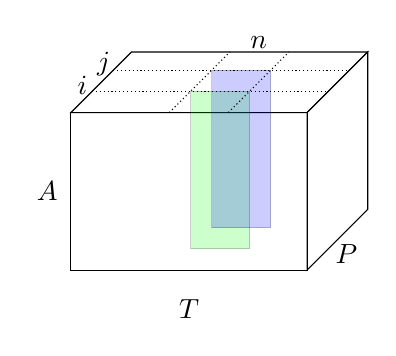
\begin{tikzpicture}
	\pgfmathsetmacro{\cubex}{3}
	\pgfmathsetmacro{\cubey}{2}
	\pgfmathsetmacro{\cubez}{2}
	\draw[black] (0,0,0) -- ++(-\cubex,0,0) -- ++(0,-\cubey,0) -- ++(\cubex,0,0) -- cycle;
	\draw[black] (0,0,0) -- ++(0,0,-\cubez) -- ++(0,-\cubey,0) -- ++(0,0,\cubez) -- cycle;
	\draw[black] (0,0,0) -- ++(-\cubex,0,0) -- ++(0,0,-\cubez) -- ++(\cubex,0,0) -- cycle;
	\draw [draw=black, fill=green,  opacity=0.2]
         (-1,0,-0.7) -- ++(-\cubex/4,0,0) -- ++(0,-\cubey,0) -- ++(\cubex/4,0,0) -- cycle;
         \draw [draw=black, fill=blue,  opacity=0.2]
         (-1,0,-1.4) -- ++(-\cubex/4,0,0) -- ++(0,-\cubey,0) -- ++(\cubex/4,0,0) -- cycle;
         \draw[densely dotted]  (-3,0,-0.7) -- (0,0,-0.7);
         \draw[densely dotted]  (-3,0,-1.4) -- (0,0,-1.4);
         \draw[densely dotted]  (-1,0,0) -- (-1,0,-2);
         \draw[densely dotted]  (-1.75,0,0) -- (-1.75,0,-2);
         \node at (-3.2,0,-0.9) {$i$};
         \node at (-3.2,0,-1.6) {$j$};
         \node at (-1.5,0,-2.3) {$n$};
	\node at (-3.3,-1) {$A$};
	\node at (-1.5,-2.5) {$T$};
	\node at (0.5, -1.8) {$P$};
	\end{tikzpicture}
	\caption{Visualization of inner loop of Algorithm \ref{alg:implicit} ($\M [\hat]{A_i}$ and $\M [\hat]{A_j} $ )}
\end{figure}


\subsection{Efficiency Comparison}

By the analysis in the previous section,  we may compare the efficiency of two methods. The speedup for both time and space complexity is dependent on variable values $A, W, P, N$ and $T$.

\bigbreak
\begin{table} \centering

\begin{tabular}{|c|c|c|}
\hline
        & Time Complexity & Space Complexity \\ \hline
Explicit Method &$A^2 W P N$+    $A^2 P^2  N$            &$A^2  N  P$ + $ATP$                   \\ \hline
Implicit Method &$A  W^2  N  P^2$                 & $A T P$                \\ \hline
Speedup          &$\frac{A(W+P)}{W^2 P}$       & $\frac{AN}{T} + 1$ \\ \hline
\end{tabular}

\caption{Time and space complexity compared between explicit and implicit methods.}
\end{table}
\bigbreak


For our experimental data, we have a brain dataset involving 61 participants, 147 time points and window size of 60. Thus, the number of windows $N = T-W+1 = 88$.  If regional based sampling is adopted, we have 268 units of area, while voxel based sampling contains around 20,000 units of area. 

With Region-based data, the speedup of implicit method over explicit method, in terms of time, is $0.8\times$ which actually decreases in speed. However, the speedup increases to $61\times$ under voxel based level.


\bigbreak

\begin{figure} \centering
\begin{tikzpicture} [scale=0.9]
\begin{axis}[
    axis lines = left,
    xlabel = $A$,
    ylabel = {Speedup},
    scaled x ticks=false
    %xticklabels={0,0 ,5000,10000,15000,20000,}
]

%Below the red parabola is defined
\addplot [
    domain=0:22000, 
    samples=100, 
    color=black,
]
{0.00305*x};
\addplot [
    domain=0:22000, 
    samples=100, 
    color=red,
    dashed
]
{1};

\addplot [color=red,mark=*] coordinates {(20000,61.111)};

\end{axis}
\end{tikzpicture}
\hskip 1pt
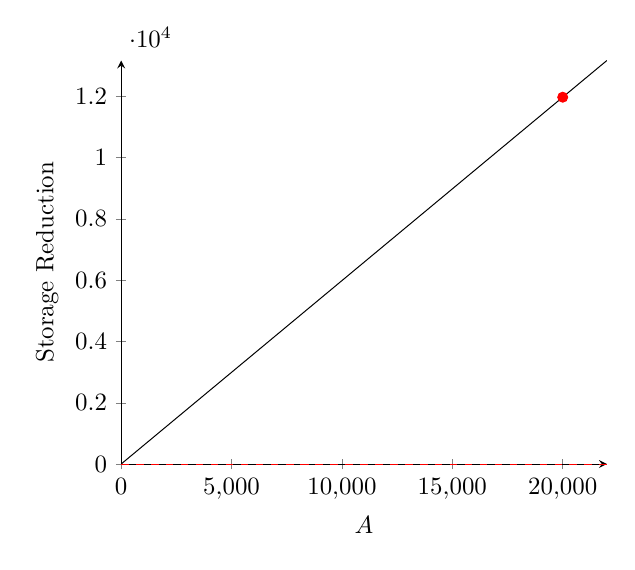
\begin{tikzpicture} [scale=0.9]
\begin{axis}[
    axis lines = left,
    xlabel = $A$,
    ylabel = {Storage Reduction},
    scaled x ticks=false,
    %scaled y ticks=false
]
%Below the red parabola is defined
\addplot [
    domain=0:22000, 
    samples=100, 
    color=black,
]
{0.5986394558*x+1};
\addplot [
    domain=0:22000, 
    samples=100, 
    color=red,
    dashed
]
{1};

\addplot [color=red,mark=*] coordinates {(20000,11973.73)};
\end{axis}
\end{tikzpicture}


\caption{Speedup in time and storage reduction corresponding to number of areas. For the experimental data, implicit method costs less time than explicit method as $A > 327$ and always requires less memory than explicit method.  The red line corresponds to value 1 to indicate when implicit method outperforms explicit method. }
\end{figure}


In terms of spatial complexity, the implicit method is 160.44 times more efficient for Region-based data, and 11,972.79 times more efficient for Voxel-based data. The implicit algorithm is always better in terms of spatial efficiency.

\subsection{Experiment}

Using the same values of  $T, W$, and $P$ as the experimental data in the previous section, we generate synthetic data with varying values of $A$ and record the corresponding experimental speedup. We plot the maximum, minimum and mean values of speedups out of 10 trials below. We also tested the performance of both methods on our machine by evaluating GFLOPS (gigaflops per second).
We see that implicit method becomes faster when $A$ exceeds approximately 350, agreeing with the theoretical analysis.
For larger $A$, we see that the experimental speedup exceeds the theoretical one (based solely on flop counts).
This deviation is attributed to the difference in memory footprints; because the memory footprint of the implicit method is smaller, it enjoys much better cache utilization than the explicit method.
At $A=2{,}500$, the memory footprint of the explicit algorithm is 24.58 GB while the footprint of the implicit algorithm is only 16.82 MB.
Because of the memory footprint of the explicit method, we could not compute empirical speedups for larger $A$. However, we have run implicit algorithm on the same synthetic data where $A$ increases to 20000, and it only takes 18.26 seconds on a single thread of 2.6 GHz Intel Core i7.


Similarly, the implicit algorithm on our real voxel based data, where $A=18225, W = 60, T = 156, P = 183$ takes 496.2MB of memory footprint and 298.8 seconds to run. It is almost impossible to store and process such data with the explicit algorithm on a normal computer.

\begin{figure}
\centering
\newcommand{\WW}{60}
\newcommand{\PP}{6}
\newcommand{\AAlim}{2500}
\begin{tikzpicture} [scale=0.9]
\begin{axis}[
    axis lines = left,
    xlabel = $A$,
    ylabel = {Speedup},
    scaled x ticks=false,
    legend pos=north west,
    legend style={at={(0,1.1)},anchor=north west,fill opacity=0.8, draw opacity=1}
    %xticklabels={0,0 ,5000,10000,15000,20000,}
]

% experimental data
\addplot[domain=0:\AAlim]
    table[x=AList,y=SpeedUpList,col sep=comma] {data/ExperimentData_Mean.csv};
    
    
% theoretical data
\addplot [
    domain=0:2500, 
    samples=2500/10, 
    color=black,
    dashed
]
{x*(\WW+\PP)/(\WW*\WW*\PP)};


\addplot [name path=A, domain=0:\AAlim, draw=none]
    table[x=AList,y=SpeedUpList,col sep=comma] {data/ExperimentData_Max.csv};
     
\addplot [name path=B,  domain=0:\AAlim, draw=none]
    table[x=AList,y=SpeedUpList,col sep=comma] {data/ExperimentData_Min.csv};
   
\addplot[pattern=north west lines, pattern color=brown!50]fill between[of=A and B, soft clip={domain=0:\AAlim}];

% crossover point    
\addplot [
    domain=0:\AAlim, 
    samples=\AAlim/10, 
    color=red,
    dashed
]
{1};

%\addplot [color=red,mark=*] coordinates {(0,0)};
\addlegendentry{Mean Experimental Speedup}
\addlegendentry{Theoretical Speedup}
\end{axis}
\end{tikzpicture}
\caption{Speedup experiment on synthetic data, the speedup is roughly linear and exceeding 1 at $300 < A < 400$, a result corresponding with the theoretical analysis. The red line corresponds to value 1 to indicate when implicit method outperforms explicit method. The shadowed area is the range of 10 experimental speedups.}
\end{figure}

\begin{figure}
\centering
\newcommand{\WW}{60}
\newcommand{\PP}{6}
\newcommand{\AAlim}{2500}
\begin{tikzpicture} [scale=0.9]
\begin{axis}[
    axis lines = left,
    xlabel = $A$,
    ylabel = {GFLOPS},
    scaled x ticks=false,
    legend pos=south east
    %xticklabels={0,0 ,5000,10000,15000,20000,}
]

% GFLOP
\addplot[domain=0:\AAlim, blue]
    table[x=AList,y=GFLOPexp,col sep=comma] {data/ExperimentData.csv};

\addplot[domain=0:\AAlim, red]
    table[x=AList,y=GFLOPimp,col sep=comma] {data/ExperimentData.csv};
   
\addlegendentry{Explicit Method GFLOP}
\addlegendentry{Implicit Method GFLOP}


%\addplot [color=red,mark=*] coordinates {(0,0)};

\end{axis}
\end{tikzpicture}
\caption{GFLOPS comparison of the same experiment on synthetic data}
\label{fig:GFLOPS}
\end{figure}


We present the raw GFLOPS in Figure \ref{fig:GFLOPS}.
We see that both methods perform at roughly the same efficiency for small values of $A$, so the speedup attained by the implicit method maps well to the theoretical comparison of the flop count.
However, for larger $A$, we see a deviation in the performance of explicit and implicit methods, which helps explain why the empirical speedup is larger.


\section{Voxel Based vs. Regional Based}

Given an efficient way of performing dimensionality reduction for Voxel-based data, our next question is, is it worth replacing Region-based analysis by Voxel-based analysis? We start off comparing the singular values and vectors resulted from the experiment above.
 
\subsection{Singular values and vectors}
Regional based activity tensor generates singular values that converge much more quickly to 0, while singular values from voxel based data are generally higher in quantity and decrease much more smoothly.  

\begin{figure} [h!] \centering
\begin{tikzpicture} [scale=0.9]
\begin{axis}[
    axis lines = left,
    ylabel = {Singular values (regional)},
    scaled x ticks=false
]

\addplot[domain=0:81]
    table[x = index, y=regSinVal, col sep=comma] {data/SingularVals.csv};

\end{axis}
\end{tikzpicture}
\hskip 1pt
\begin{tikzpicture} [scale=0.9]
\begin{axis}[
    axis lines = left,
    ylabel = {Singular values (voxel)},
    scaled x ticks=false,
]
\addplot[domain=0:81]
    table[x = index, y=voxSinVal, col sep=comma] {data/SingularVals.csv};

\end{axis}
\end{tikzpicture}

\caption{Singular values computed from two techniques.}
\end{figure}


The singular vectors from regional based data seems like random numbers around 0 without special patterns, while those from voxel based data contains several extreme values far from 0. Since x-axis corresponds to participants $P$, these spikes indicates that voxel based data contains some outstanding tendency for different participants. 


\begin{figure} [h!] \centering
\begin{tikzpicture} [scale=0.9]
\begin{axis}[
    axis lines = left,
    ylabel = {Singular vectors (regional)},
    scaled x ticks=false
]

\addplot[domain=0:81, red]
    table[x = index, y=u0, col sep=comma] {data/RegSinVecs.csv};
\addplot[domain=0:81, blue]
    table[x = index, y=u1, col sep=comma] {data/RegSinVecs.csv};
\addplot[domain=0:81, yellow]
    table[x = index, y=u2, col sep=comma] {data/RegSinVecs.csv};
\addplot[domain=0:81, green]
    table[x = index, y=u3, col sep=comma] {data/RegSinVecs.csv};
\addplot[domain=0:81, black]
    table[x = index, y=u4, col sep=comma] {data/RegSinVecs.csv};
    
\end{axis}
\end{tikzpicture}
\hskip 1pt
\begin{tikzpicture} [scale=0.9]
\begin{axis}[
    axis lines = left,
    ylabel = {Singular vectors (voxel)},
    scaled x ticks=false,
]

\addplot[domain=0:81, red]
    table[x = index, y=u0, col sep=comma] {data/VoxSinVecs.csv};
\addplot[domain=0:81, blue]
    table[x = index, y=u1, col sep=comma] {data/VoxSinVecs.csv};
\addplot[domain=0:81, yellow]
    table[x = index, y=u2, col sep=comma] {data/VoxSinVecs.csv};
\addplot[domain=0:81, green]
    table[x = index, y=u3, col sep=comma] {data/VoxSinVecs.csv};
\addplot[domain=0:81, black]
    table[x = index, y=u4, col sep=comma] {data/VoxSinVecs.csv};

\end{axis}
\end{tikzpicture}

\caption{Singular vectors corresponding to the 5 biggest singular values computed from two techniques.}
\end{figure}


\newpage
\subsection{Individual Classification}

One of the scientific questions we try to answer is classification over participants $P$. The data we use for this task contains 61 participants each testing 3 tasks, thus $P = 183$. We label 61 individual participants and processed the data using our implicit algorithm to get a matrix of left singular vectors with dimension $183 \times 183$. To get fair accuracy, we use stratified 3-fold cross-validation to divide the data into 3 parts, each with 61 distinguished labels of participants. Then we iteratively train machine learning models based on two of three parts and use the left-out part of data to valid model accuracy. Our final accuracy is calculated as the average of the three validation scores. 

We observe higher classification accuracy for Voxel-based data in machine learning models. The most successful model is GBDT (Gradient Boosting Decision Tree), which achieves 83.6\% classification accuracy on voxel data while only 49.7\% on regional data. It is a sheer win for voxel data to classify individual participants.

\begin{table} \centering

\begin{tabular}{|c|c|c|}
\hline
        & Trained on Regonal Data & Trained on Voxel Data \\ \hline
Dummy Classifer &.016        & .016              \\ \hline
Random Forest &.007           & .289               \\ \hline
GBDT         &0.497      & .836 \\ \hline
KNN        &.011     & .032 \\ \hline      
\end{tabular}

\caption{Individual classification accuracy trained on regional and voxel data using Random Forest, Gradient Boosting Decision Trees and K-Nearest Neighbors classifiers.}
\end{table}

We also implemented other models such as Supporting Vector Machines \cite{SVM} and Generalized Linear Regression. However they failed to converge due to the limited number of	 samples within classes.



\subsection{Farm/Nonfarm Worker Classification}

Using the same data as the previous section, we divide the 61 participants into 22 farm workers and 39 non-farm workers. Then we label the total 183 cases into two classes before a stratified 3 fold cross validation. However, the result of this task fails to prove the advantage of voxel based data over regional data. The classification accuracy for both form of data are close enough to each other. 




\begin{table} \centering

\begin{tabular}{|c|c|c|}
\hline
        & Trained on Regonal Data & Trained on Voxel Data \\ \hline
Dummy Classifer &.639        & .639              \\ \hline
Random Forest &.622           & .743              \\ \hline
GBDT         &0.852      & .857 \\ \hline
KNN        &.546     & .595 \\ \hline      
\end{tabular}

\caption{Farm/NonFarm Workers classification accuracy trained on regional and voxel data using Random Forest, Gradient Boosting Decision Trees and K-Nearest Neighbors classifiers.}
\end{table}


\subsection{Clustering}

Besides supervised classification, we also tried to cluster one of the three tasks in an unsupervised way. After preprocessing with implicit algorithm, we have a $61 \times 61$ matrix of singular vectors. KMeans clustering on these singular vectors can separate them into two groups. Then we compare the result with Farm/Nonfarm worker labels to compute target similarity between them. It turns out that voxel based data seems hard for Kmeans to find any useful pattern. On the other side, regional data reaches its maximum as we use two leading left singular vectors, but fails to work as the number of singular vectors increases.


\begin{figure}  \centering
\graphicspath{ {data/} }

\includegraphics[scale=0.5]{KMeans}
\caption{Farm/Non-farm worker classification accuracy}
\end{figure}


\section{Conclusion}

So far we have developed an efficient algorithm in performing SVD on correlation activity tensors. The speedup and storage reduction are significant both theoretically and practically. Using an efficient algorithm, we have performed several experiments and found that using voxel based data answers individual classification problem more accurately than region-based data.  More experiments must be made in order to gain comprehensive insight of the advantage of voxel data, and we believe our implicit algorithm lays a basis for the potential research in the future. 

\newpage
\bibliographystyle{unsrt}
\bibliography{paper.bib}



\end{document}









